%%%%%%%%%%%%%%%%%%%%%%%%%%%%%%%%% METADADOS %%%%%%%%%%%%%%%%%%%%%%%%%%%%%%%%%%%%

\title[The shortened title]{Tópicos em Paralelização de Compiladores:\\ um estudo de caso no GCC}
%\subtitle{The (optional) subtitle}

\author[Authors Name]{Giuliano Belinassi}

%\institute[USP]{\textbf{Workshop Name} \\ Computer Science Department \\ IME USP}
\institute[USP]{\textbf{Orientador: Alfredo Goldman} \\ Departmentamento de Ciência da Computação \\ IME USP}

\date{17 de Junho de 2019}

% Coloca a imagem no fundo da página de título
%\bgimage{\includegraphics[width=\paperwidth]{fundo_predios_e_grafo}}

% Logotipos no rodapé da página de título
%\logos{
%  \hfil\hfil\includegraphics[width=.1\textwidth]{usp-logo}\hfil%
%  \raisebox{-.0103\paperheight}{\includegraphics[height=.0932\paperheight]{interscity-logo}}\hfil%
%  \raisebox{-.033\paperheight}{\includegraphics[width=.07\textwidth,trim=0 230 0 0,clip]{ime-logo}}\hfil\hfil
%}
%
\logos{
  \hfil\hfil\includegraphics[width=.1\textwidth]{usp-logo}\hfil%
%  \raisebox{-.0103\paperheight}{\includegraphics[height=.0932\paperheight]{interscity-logo}}\hfil%
%  \raisebox{-.00517\paperheight}{
\includegraphics[height=.057\paperheight]{cnpq-logo}}\hfil%
  \raisebox{-.02\paperheight}{
\includegraphics[height=.1035\paperheight]{capes-logo}}\hfil\hfil\strut%
%  \includegraphics[height=.044\paperheight]{fapesp-logo}\hfil\hfil
}

% Usado para criar o qrcode com o endereço da apresentação
%\presentationurl{http://interscity.org}

% Inclui o qrcode no sumário da apresentação
%\includeqrcodeintoc

% O slide de sumário pode ser dividido em colunas; o parâmetro
% determina após qual o número da seção fazer a quebra de coluna
% (use zero para uma coluna ou simplesmente omita este comando).
\toccolumns{4}


%%%%%%%%%%%%%%%%%%%%%%%%%%%%%%%%%%%%%%%%%%%%%%%%%%%%%%%%%%%%%%%%%%%%%%%%%%%%%%%%
%%%%%%%%%%%%%%%%%%%%%%%%%%%% INÍCIO DA APRESENTAÇÃO %%%%%%%%%%%%%%%%%%%%%%%%%%%%
%%%%%%%%%%%%%%%%%%%%%%%%%%%%%%%%%%%%%%%%%%%%%%%%%%%%%%%%%%%%%%%%%%%%%%%%%%%%%%%%

% É complicado colocar uma imagem de fundo, os logos das agências e
% o conteúdo "normal" do slide de título sem que as coisas fiquem
% bagunçadas, então definimos um comando para gerar o slide de título
\customtitlepage

% Slide com o qrcode
%\showqrcode

\begin{frame}{Objetivos da Pesquisa}
    \begin{itemize}
        \item Paralelização de um compilador internamente
        \begin{itemize}
            \item Sem modificar a estrutura da compilação
            \item Permitindo explorar paralelismo dentro de arquivos
        \end{itemize}
        \item Revisão de técnicas para a paralelização de Compiladores
        \item[]
        \item Consequências
        \begin{itemize}
            \item Compilações mais rápidas
            \item Economia de energia
            \item Integração Contínua mais responsiva
            \item Alternativa ao \textit{Link Time Optimization} (LTO)
        \end{itemize}
    \end{itemize}
\end{frame}

\begin{frame}{Visão Geral}
  \overview
\end{frame}

\section{Introdução}

\begin{frame}{Introdução}
  \begin{itemize}
    \item Compiladores-Otimizadores são softwares enormes e complexos
        \begin{itemize}
            \item Exemplos ainda com desenvolvimento ativo: GCC (1987), Clang (2007)
            \item Majoritariamente sequenciais
        \end{itemize}
    \item Uso de recursos de programação como \texttt{templates}
    \item Geração automática de arquivos grandes
        \begin{itemize}
            \item \texttt{gimple-match.c}: {\color{red}{100358 linhas}} de C++ (GCC 10.0.0)
        \end{itemize}
  \end{itemize}
\end{frame}


\begin{frame}{Introdução}
    Paralelismo em compiladores:
    \begin{itemize}
        \item Normalmente com \texttt{make -j}
            \begin{itemize}
                \item Granularidade por arquivo
                \item Modelo clássico de compilação
            \end{itemize}
    \end{itemize}
\end{frame}

\begin{frame}{Introdução}
\begin{figure}
\tikzstyle{block} = [rectangle, draw, fill=white,
    text width=6em, text centered, rounded corners, node distance=1cm and 2cm, auto, minimum height=2em]
\tikzstyle{line} = [draw, -latex]
\tikzstyle{cloud} = [draw, ellipse,fill=white, node distance=1cm,
    minimum height=2em]
\begin{center}
\scalebox{0.7}{
\begin{tikzpicture}
    % Place nodes
    \node [block]                         (make)   {Makefile};
    \coordinate[below=of make]            (c);
    \node [block, left=of c]              (fonte1) {fonte1.c};
    \node [block, right=of fonte1]        (fonte2) {fonte2.cpp};
    \node [block, right=of fonte2]        (fonte3) {fonte3.f90};

    \node [block, below=of fonte1]        (gcc)      {gcc};
    \node [block, below=of fonte2]        (g++)      {g++};
    \node [block, below=of fonte3]        (gfortran) {gfortran};

    \node [block, below=of gcc]           (objeto1) {objeto1.o};
    \node [block, below=of g++]           (objeto2) {objeto2.o};
    \node [block, below=of gfortran]      (objeto3) {objeto3.o};

    \node [block, below=of objeto2]       (ld) {LD};

    \node [block, below=of ld]            (bin) {Executável};

    % Draw edges
    \draw[->]    ([xshift=-0.7em] make.south)   -- (fonte1.north);
    \draw[->]    (make.south)   -- (fonte2.north);
    \draw[->]    ([xshift=+0.7em] make.south)   -- (fonte3.north);

    \draw[->]    (fonte1.south)   -- (gcc.north);
    \draw[->]    (fonte2.south)   -- (g++.north);
    \draw[->]    (fonte3.south)   -- (gfortran.north);

    \draw[->]    (gcc.south)   -- (objeto1.north);
    \draw[->]    (g++.south)   -- (objeto2.north);
    \draw[->]    (gfortran.south)   -- (objeto3.north);

    \draw[->]    (objeto1.south)   -- ([xshift=-0.7em]ld.north);
    \draw[->]    (objeto2.south)   -- (ld.north);
    \draw[->]    (objeto3.south)   -- ([xshift=+0.7em]ld.north);

    \draw[->]    (ld.south)   -- (bin.north);


\end{tikzpicture}
}
\end{center}
\caption{Processo clássico de compilação de um programa.}
\label{fig:classical_build}
\end{figure}
\end{frame}

\begin{frame}{Introdução}
    \begin{itemize}
        \item O que acontece se há alguns arquivos grandes no projeto?
        \begin{itemize}
            \item Gargalo na compilação
            \item Maior gasto de energia
            \item Exemplos
                \begin{itemize}
                    \item O próprio GCC
                    \item Relatos similares em projetos internos \citep{mailgcc}
                \end{itemize}
        \end{itemize}
    \end{itemize}
\end{frame}

\begin{frame}{Introdução}
    \begin{itemize}
        \item Experimento 1
        \begin{itemize}
            \item Compilação do GCC em uma máquina com $4\times$ AMD Opteron 6376
                \begin{itemize}
                    \item $4 \times 16 = 64$ núcleos
                \end{itemize}
            \item \textit{Bootstrap} desligado
            \item Coletado os {\color{blue}{tempos de compilação}} de {\color{red}{cada arquivo}}
            \item Coletado a {\color{blue}{soma da potência instantânea}} fornecida a
                {\color{red}{cada processador}}
                \begin{itemize}
                    \item Sensor AMD \texttt{fam15h\_power}
                    \item $\Delta t = 5ms$
                \end{itemize}
        \end{itemize}
    \end{itemize}
\end{frame}

\begin{frame}
    Paralelismo com Makefile
    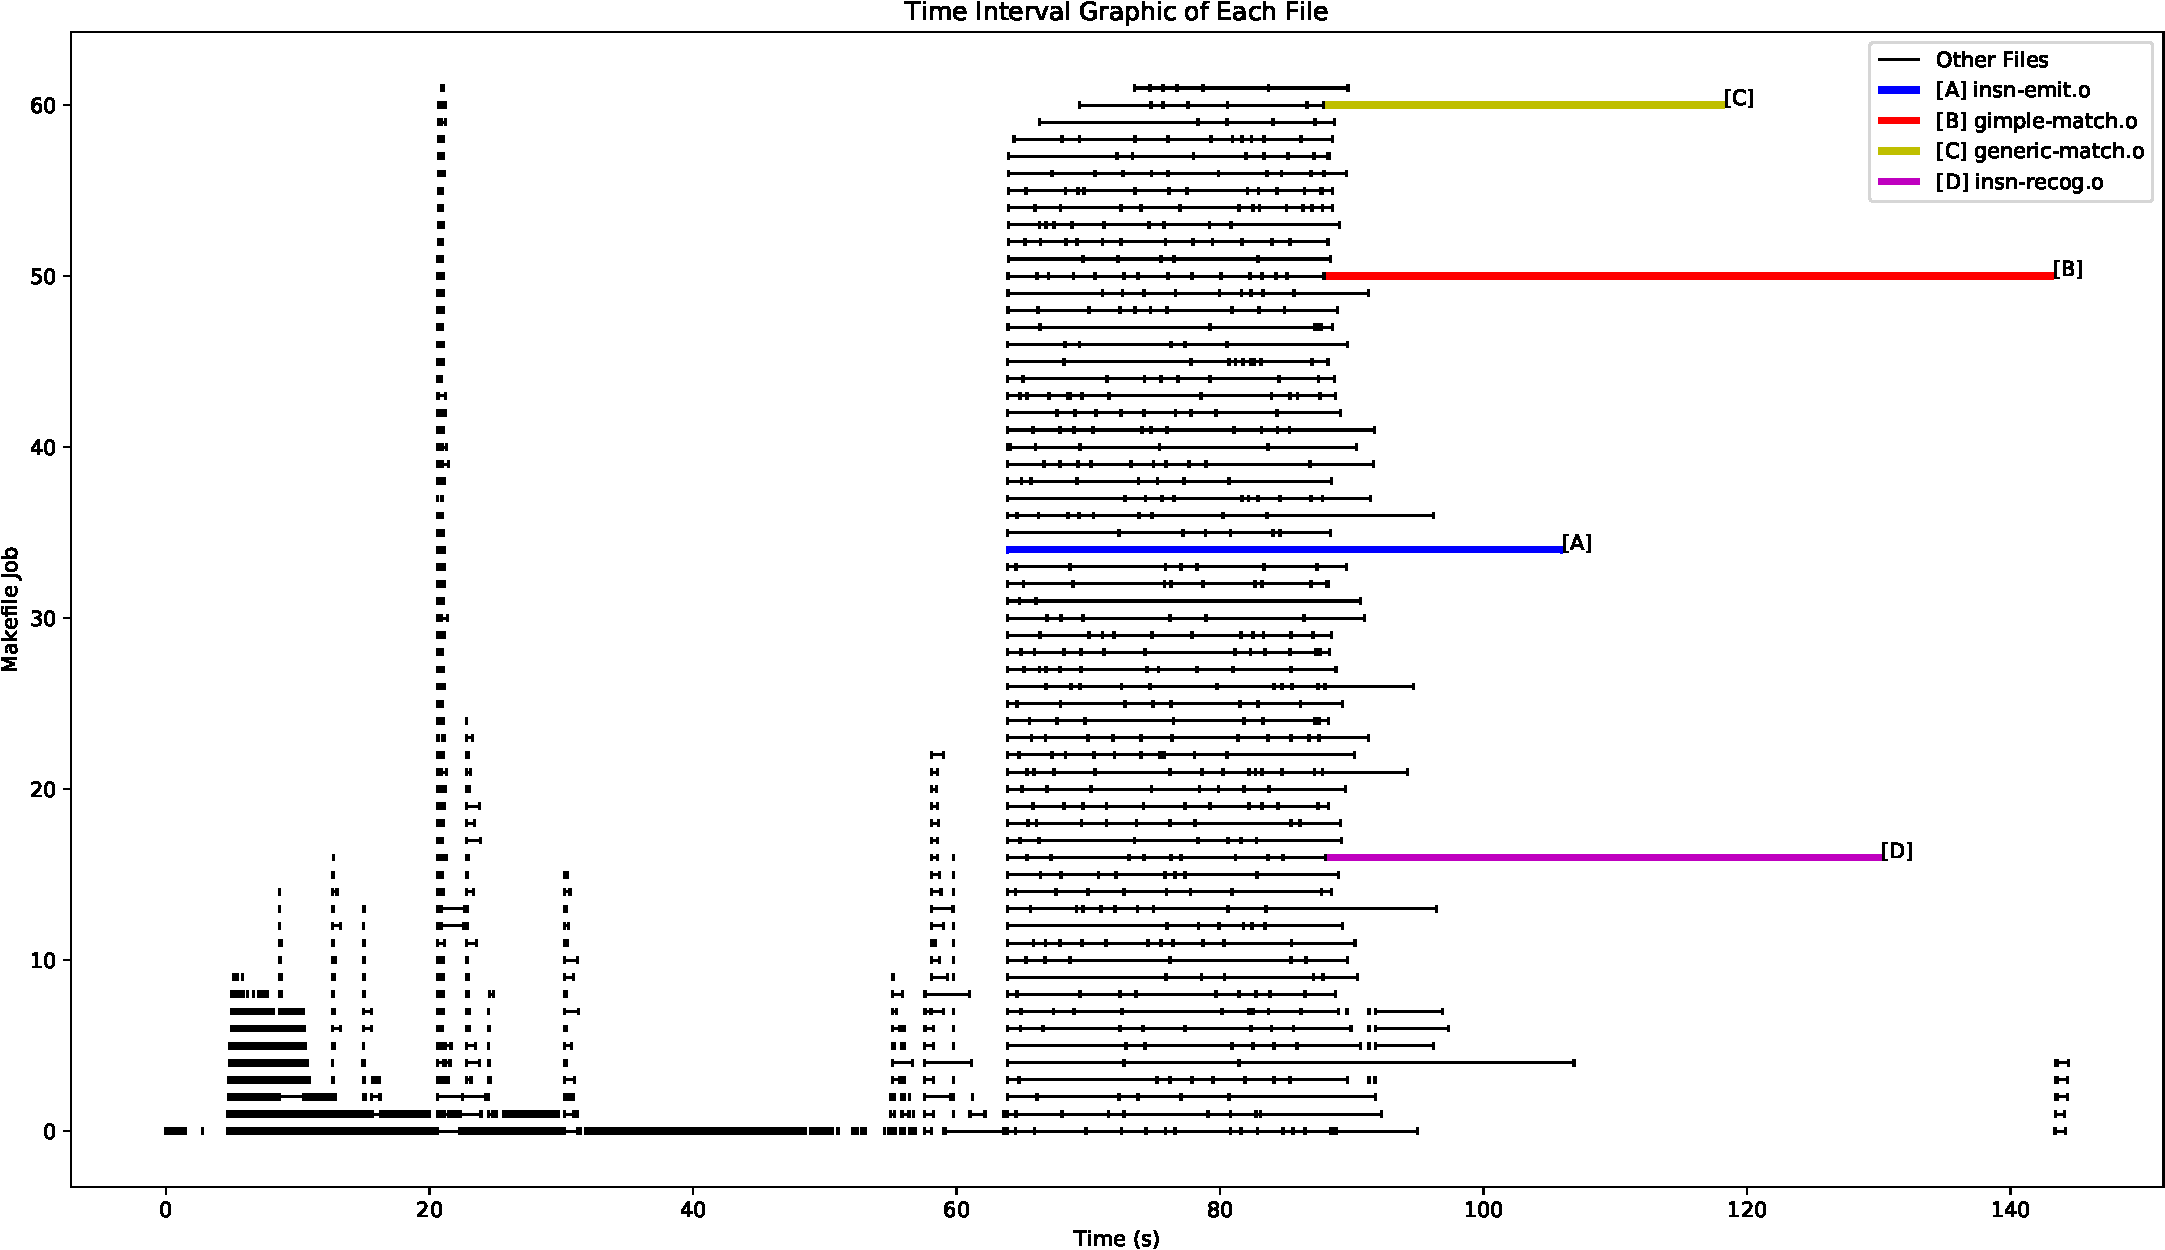
\includegraphics[width=0.9\paperwidth]{gcc_timer_classic_crop.pdf}
    %   \captionof{figure}{Tempo corrido na compilação do GCC em um processador de
    %64 núcleos. \textbf{Sem} LTO, sem \textit{Bootstrap}.}
    \label{fig:analysis_classical}
\end{frame}

\begin{frame}
    Paralelismo com Makefile
    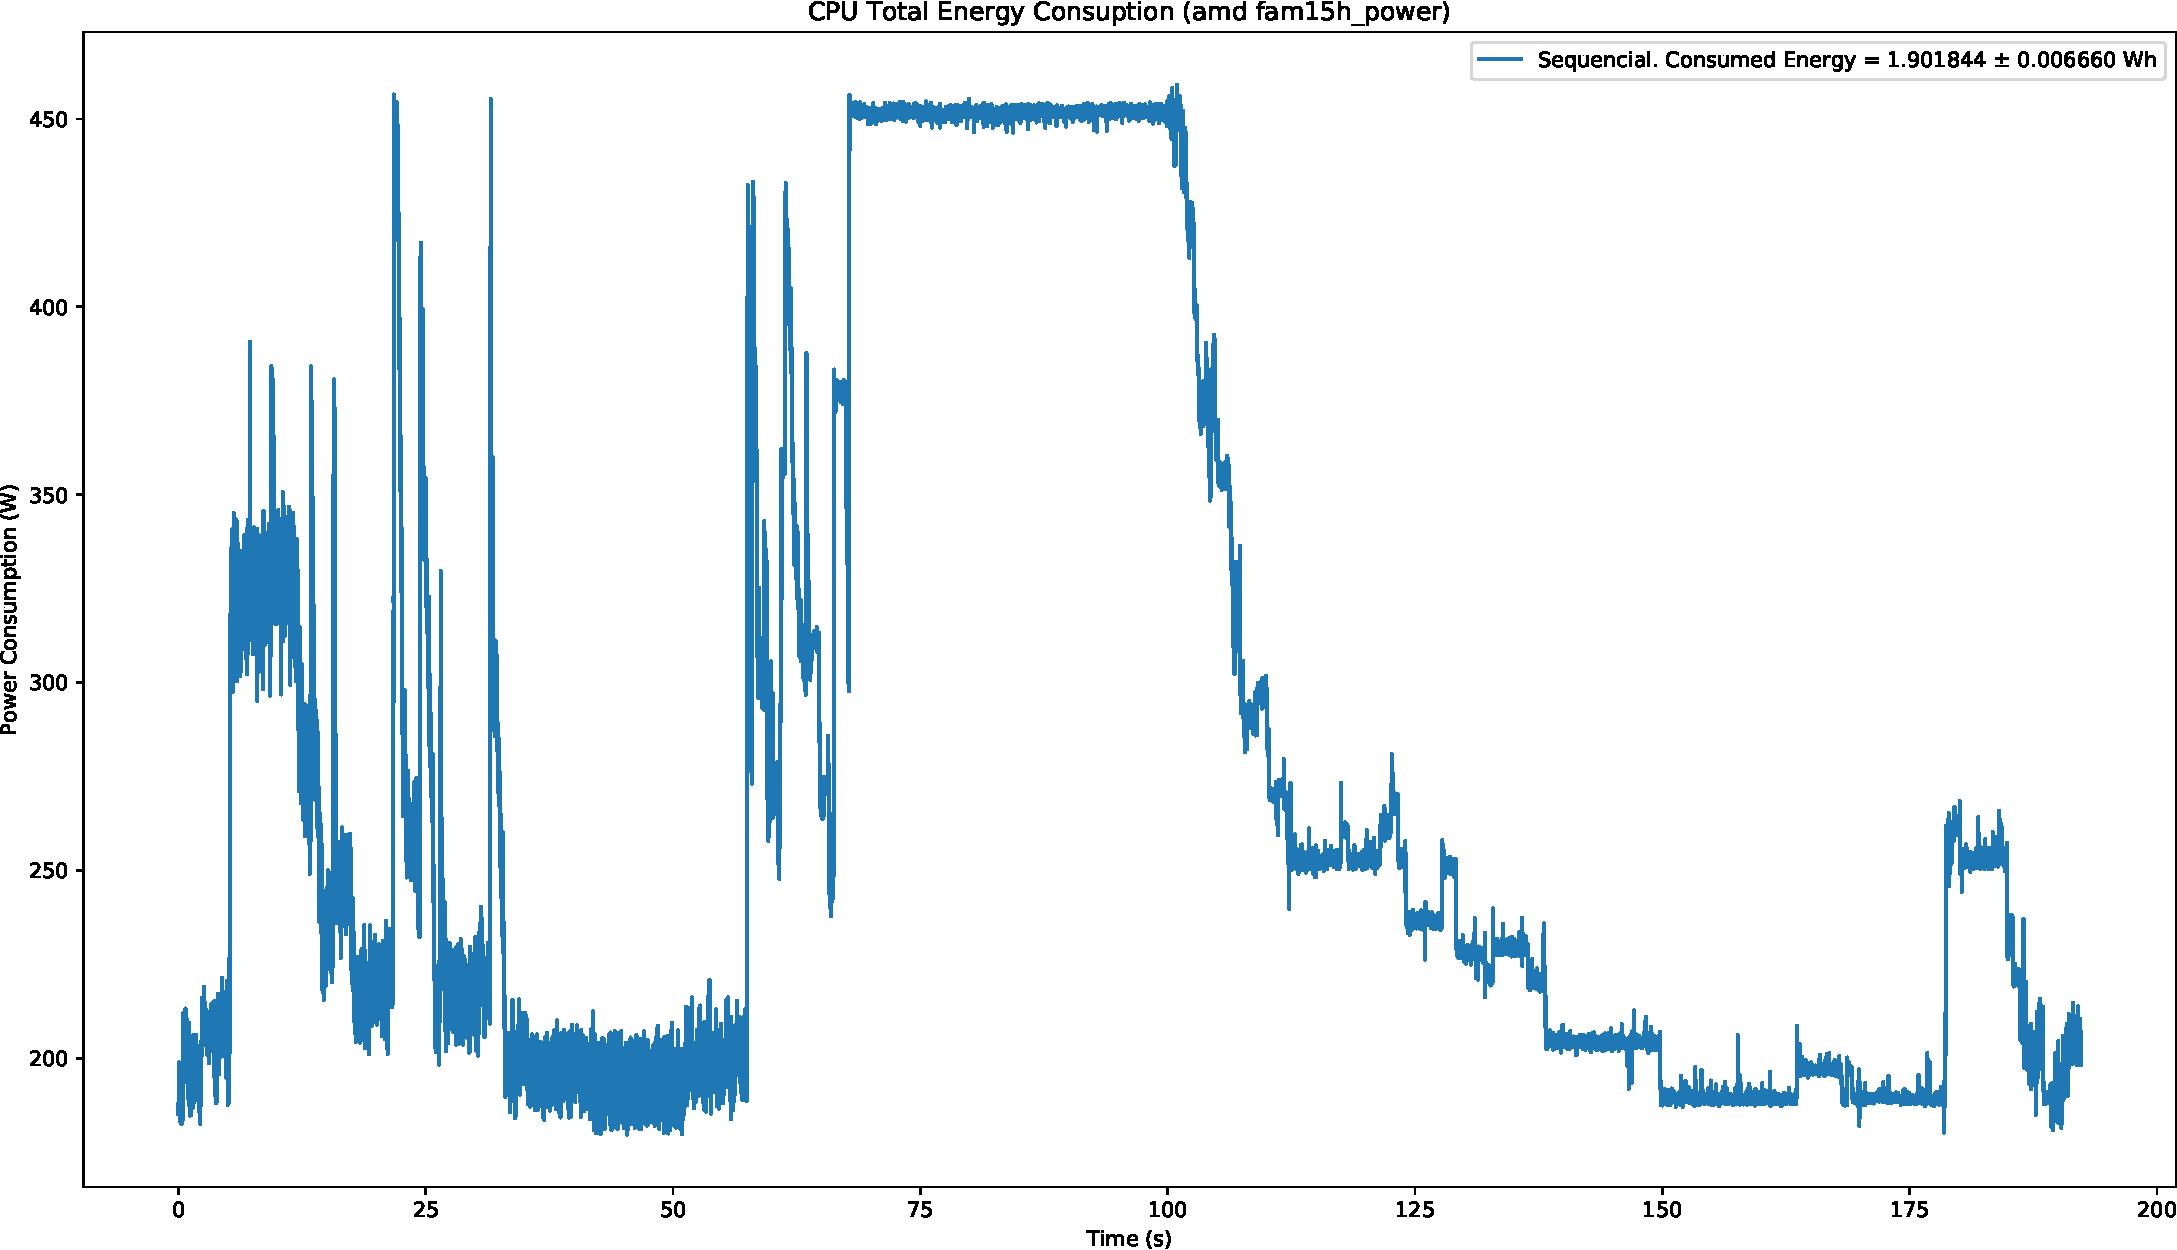
\includegraphics[width=0.9\paperwidth]{sensors-crop.pdf}
    %   \captionof{figure}{Tempo corrido na compilação do GCC em um processador de
    %64 núcleos. \textbf{Sem} LTO, sem \textit{Bootstrap}.}
    \label{fig:analysis_classical}
\end{frame}

\begin{frame}
    \begin{itemize}
        \item Como demonstrado, o \texttt{make -j} não é suficiente!
        \item[]
        \begin{itemize}
            \item Isso levanta as seguintes questões de pesquisas:
            \begin{description}
                \item[\textit{QP1}] Em que pontos um compilador pode usufruir de paralelismo?
                \item[\textit{QP2}] Qual é o ganho de tempo ao paralelizar um compilador?
                \item[\textit{QP3}] Quanta energia é economizada ao paralelizar um compilador?
            \end{description}
        \end{itemize}
    \end{itemize}
\end{frame}



\begin{frame}{Visão Geral}
  \overview
\end{frame}

\section{Trabalhos Relacionados}

\begin{frame}{Trabalhos Relacionados}
    \begin{itemize}
        \item Pesquisa de paralelismo em compiladores é majoritariamente destinada a compiladores que paralelizam
        \item[]
        \item Existem duas áreas relacionadas a paralelização de compiladores:
        \begin{itemize}
            \item Análise de texto em paralelo (análise léxica e sintática)
            \item Análise de fluxo de dados e controle em paralelo
        \end{itemize}
    \end{itemize}
\end{frame}

\begin{frame}{Trabalhos Relacionados}
    Análise Léxica e Sintática em Paralelo
    \begin{itemize}
        \item \cite{Mickunas:1978:PCM:800127.804105} propôs uma paralelização do algoritmo LR(0)
            \begin{itemize}
                \item Particiona o arquivo de entrada arbitrariamente
                \item Executa um analisador LR(0) em cada partição
                \item Se o analisador encontrar uma ambiguidade, envia a sua entrada para o analisador à sua esquerda
            \end{itemize}
    \end{itemize}
\end{frame}

\begin{frame}{Trabalhos Relacionados}
    Compilação em Paralelo
    \begin{itemize}
        \item \cite{vandevoorde1988parallel} implementou um compilador C paralelo
            \begin{itemize}
                \item Analisador Sintático em paralelo ao Analisador Léxico
                    \begin{itemize}
                        \item Os \textit{tokens} são alimentados através de um \textit{pipeline}
                    \end{itemize}
                \item O Analisador Sintático executa em paralelo a cada expressão
                \item[]
                \item Supõe que todas as declarações de funções estão no cabeçalho do arquivo
                \item {\color{red}{Não discute otimização}}
            \end{itemize}
    \end{itemize}
\end{frame}

\begin{frame}{Trabalhos Relacionados}
    Compilação em Paralelo
    \begin{itemize}
        \item \cite{wortman1992} implementou um compilador Modula-2+ em paralelo
            \begin{itemize}
                \item Analisador Léxico encontra funções no código
                \item Alimenta as funções através de uma fila de prioridade produtor-consumidor
                \item Procede com a compilação das funções em paralelo
                \item Propõe estratégias para solucionar os problemas de símbolos não definidos
                    \begin{itemize}
                        \item Uma \textit{thread} viu um símbolo que a outra precisa
                    \end{itemize}
                \item Procede com a geração de código em paralelo para cada função
                \item[]
                \item {\color{red}{Não discute otimização}}
            \end{itemize}
    \end{itemize}
\end{frame}

\begin{frame}{Trabalhos Relacionados}
    Otimização em Paralelo 

    \begin{itemize}
        \item \cite{Lee1994} propõem uma análise de controle de fluxo em paralelo
            \begin{itemize}
                \item Particionam o grafo em regiões conexas.
                \item Executam
            \end{itemize}
    \end{itemize}

\end{frame}

\begin{frame}{Trabalhos Relacionados}
    Existem dois conjuntos de otimizações que podem ser aplicadas em uma função do código:
  \begin{itemize}
    \item \textit{Intra Procedural}
        \begin{itemize}
            \item Podem ser aplicadas sem observar as interações com as demais funções
        \end{itemize}
    \item \textit{Inter Procedural}
        \begin{itemize}
            \item É necessário analisar as interações com as demais funções
            \item Processo conhecido como \textit{Inter Process Analysis} (IPA)
        \end{itemize}
    \item[]
    \item Note que estes dois conjuntos são disjuntos (intersecção é vazia)
  \end{itemize}
\end{frame}

%\begin{frame}{Introdução e Definições}
%  Um compilador normalmente é dividido em três etapas
%  \begin{itemize}
%    \item \textit{Front End}
%        \begin{itemize}
%            \item Responsável por interagir com o programa na linguagem $A$
%            \item Análise Léxica e Sintática
%            \item Exemplo: converte um código C para uma representação interna em árvores
%        \end{itemize}
%    \item \textit{Middle End}
%        \begin{itemize}
%            \item Responsável por efetuar \textit{otimizações independentes de arquitetura} no código original
%        \end{itemize}
%    \item \textit{Back End}
%        \begin{itemize}
%            \item Responsável por \textit{traduzir} a representação interna para $B$
%            \item Otimização dependentes de arquitetura, geração de código
%        \end{itemize}
%  \end{itemize}
%\end{frame}
%\begin{frame}{Introdução e Definições}
%\begin{figure}
%\tikzstyle{block} = [rectangle, draw, fill=white,
%    text width=6em, text centered, rounded corners, node distance=1cm and 1cm, auto, minimum height=2em]
%\tikzstyle{line} = [draw, -latex]
%\tikzstyle{cloud} = [draw, ellipse,fill=white, node distance=2cm,
%    minimum height=2em]

%\begin{center}
%\scalebox{1.0}{
%    \begin{tikzpicture}
%    % Place nodes
%    \begin{scope}{node distance = 1cm and 1cm}
%    \node [block]                      (front_c)    {Frontend C};
%    \node [block, below=of front_c]    (front_cpp)  {Frontend C++};
%    \node [block, below=of front_cpp]  (front_fort) {Frontend Fortran};
%    \node [block, right=of front_cpp]  (middle)     {Middle End};
%    \node [block, right=of middle]     (back_x86)   {Backend x86};
%    \node [block, above=of back_x86]   (back_arm)   {Backend ARM};
%    \node [block, below=of back_x86]   (back_ppc)   {Backend PPC};
%
%
%    \coordinate [left=of front_c]    (c_code);
%    \coordinate [left=of front_cpp]  (cpp_code);
%    \coordinate [left=of front_fort]  (fort_code);
%
%    \coordinate [right=of back_x86] (x86_code);
%    \coordinate [right=of back_arm] (arm_code);
%    \coordinate [right=of back_ppc] (ppc_code);
%    \end{scope}
%
%    % Draw edges
%    \draw[->]    (front_c.east)     to [out=0,in=180] ([yshift=0.5em]  middle.west);
%    \draw[->]    (front_cpp.east)   to [out=0,in=180] (middle.west);
%    \draw[->]    (front_fort.east)  to [out=0,in=180] ([yshift=-0.5em] middle.west);
%
%    \draw[->]    ([yshift=-0.5em] middle.east)  to [out=0,in=180] (back_ppc.west);
%    \draw[->]    (middle.east)                  to [out=0,in=180] (back_x86.west);
%    \draw[->]    ([yshift=0.5em] middle.east)   to [out=0,in=180] (back_arm.west);
%
%\end{tikzpicture}
%}
%\end{center}
%
%\caption{Arquitetura de um compilador.}
%\label{fig:compiler_arch}
%\end{figure}
%\end{frame}

\begin{frame}{Introdução e Definições}
    Existem dois conjuntos de otimizações que podem ser aplicadas em uma função do código:
  \begin{itemize}
    \item \textit{Intra Procedural}
        \begin{itemize}
            \item Podem ser aplicadas sem observar as interações com as demais funções
        \end{itemize}
    \item \textit{Inter Procedural}
        \begin{itemize}
            \item É necessário analisar as interações com as demais funções
            \item Processo conhecido como \textit{Inter Process Analysis} (IPA)
        \end{itemize}
    \item[]
    \item Note que estes dois conjuntos são disjuntos (intersecção é vazia)
  \end{itemize}
\end{frame}

\section{Objetivos do Trabalho}

\begin{frame}{Objetivos da Pesquisa}
    \begin{itemize}
        \item Paralelização de um compilador internamente
        \begin{itemize}
            \item Sem modificar a estrutura da compilação
            \item Permitindo explorar paralelismo dentro de arquivos
        \end{itemize}
        \item Revisão de técnicas para a paralelização de Compiladores
        \item[]
        \item Consequências
        \begin{itemize}
            \item Compilações mais rápidas
            \item Economia de energia
            \item Integração Contínua mais responsiva
            \item Alternativa ao \textit{Link Time Optimization} (LTO)
        \end{itemize}
    \end{itemize}
\end{frame}



\begin{frame}[standout]
    Por quê?
\end{frame}

\section{Problematização}

\begin{frame}{Problematização}
  \begin{itemize}
    \item Compiladores-Otimizadores são softwares enormes e complexos
        \begin{itemize}
            \item Exemplos ainda com desenvolvimento ativo: GCC (1987), Clang (2007)
            \item Majoritariamente sequenciais
        \end{itemize}
    \item Uso de recursos de programação como \texttt{templates}
    \item Geração automática de arquivos grandes
        \begin{itemize}
            \item \texttt{gimple-match.c}: 100358 linhas de C++ (GCC 10.0.0)
        \end{itemize}
  \end{itemize}
\end{frame}
    
\begin{frame}{Problematização}
    Paralelismo com o GCC:
    \begin{itemize}
        \item Com \texttt{Makefiles}
            \begin{itemize}
                \item Granularidade por arquivo
                \item Modelo clássico de compilação
            \end{itemize}
        \item Através do \textit{Link Time Optimization} (LTO)
            \begin{itemize}
                \item Faz otimizações mais agressivas
                \item Muda como o processo de compilação é realizado
                \item Não confiável em vários casos
                \item Gera código menos eficiente em alguns casos
            \end{itemize}
    \end{itemize}
\end{frame}


\begin{frame}[standout]
    Usando \texttt{Makefiles}
\end{frame}

\begin{frame}{Processo de Compilação Clássico}
\begin{figure}
\tikzstyle{block} = [rectangle, draw, fill=white,
    text width=6em, text centered, rounded corners, node distance=1cm and 2cm, auto, minimum height=2em]
\tikzstyle{line} = [draw, -latex]
\tikzstyle{cloud} = [draw, ellipse,fill=white, node distance=1cm,
    minimum height=2em]
\begin{center}
\scalebox{0.7}{
\begin{tikzpicture}
    % Place nodes
    \node [block]                         (make)   {Makefile};
    \coordinate[below=of make]            (c);
    \node [block, left=of c]              (fonte1) {fonte1.c};
    \node [block, right=of fonte1]        (fonte2) {fonte2.cpp};
    \node [block, right=of fonte2]        (fonte3) {fonte3.f90};

    \node [block, below=of fonte1]        (gcc)      {gcc};
    \node [block, below=of fonte2]        (g++)      {g++};
    \node [block, below=of fonte3]        (gfortran) {gfortran};

    \node [block, below=of gcc]           (objeto1) {objeto1.o};
    \node [block, below=of g++]           (objeto2) {objeto2.o};
    \node [block, below=of gfortran]      (objeto3) {objeto3.o};

    \node [block, below=of objeto2]       (ld) {LD};

    \node [block, below=of ld]            (bin) {Executável};

    % Draw edges
    \draw[->]    ([xshift=-0.7em] make.south)   -- (fonte1.north);
    \draw[->]    (make.south)   -- (fonte2.north);
    \draw[->]    ([xshift=+0.7em] make.south)   -- (fonte3.north);

    \draw[->]    (fonte1.south)   -- (gcc.north);
    \draw[->]    (fonte2.south)   -- (g++.north);
    \draw[->]    (fonte3.south)   -- (gfortran.north);

    \draw[->]    (gcc.south)   -- (objeto1.north);
    \draw[->]    (g++.south)   -- (objeto2.north);
    \draw[->]    (gfortran.south)   -- (objeto3.north);

    \draw[->]    (objeto1.south)   -- ([xshift=-0.7em]ld.north);
    \draw[->]    (objeto2.south)   -- (ld.north);
    \draw[->]    (objeto3.south)   -- ([xshift=+0.7em]ld.north);

    \draw[->]    (ld.south)   -- (bin.north);


\end{tikzpicture}
}
\end{center}
\caption{Processo clássico de compilação de um programa.}
\label{fig:classical_build}
\end{figure}
\end{frame}

\begin{frame}
    Paralelismo com Makefile
    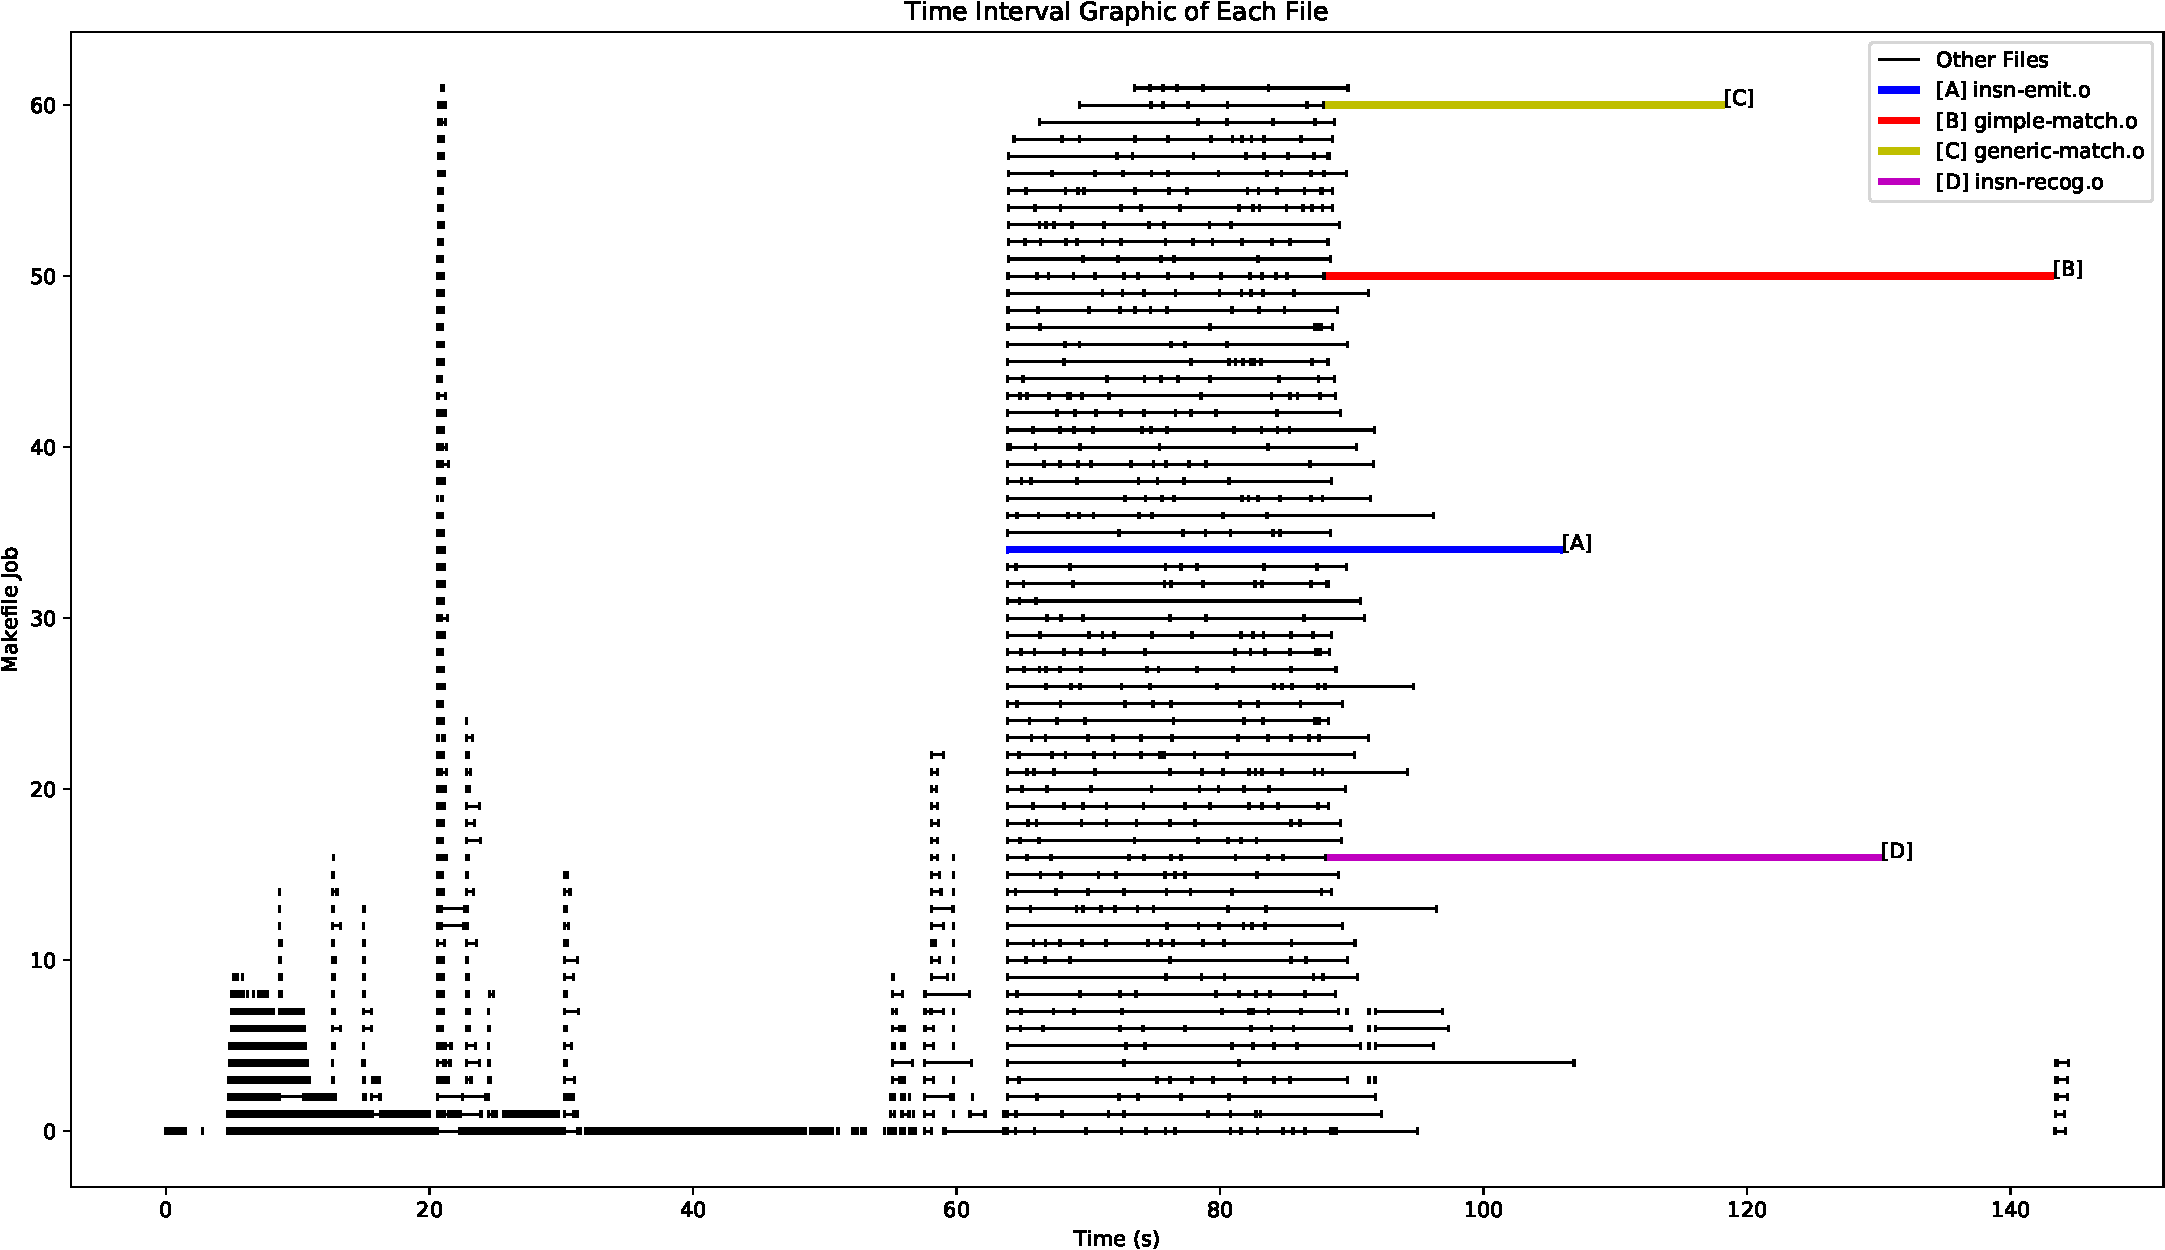
\includegraphics[width=0.9\paperwidth]{gcc_timer_classic_crop.pdf}
    %   \captionof{figure}{Tempo corrido na compilação do GCC em um processador de
    %64 núcleos. \textbf{Sem} LTO, sem \textit{Bootstrap}.}
    \label{fig:analysis_classical}
\end{frame}

\begin{frame}
    Paralelismo com Makefile
    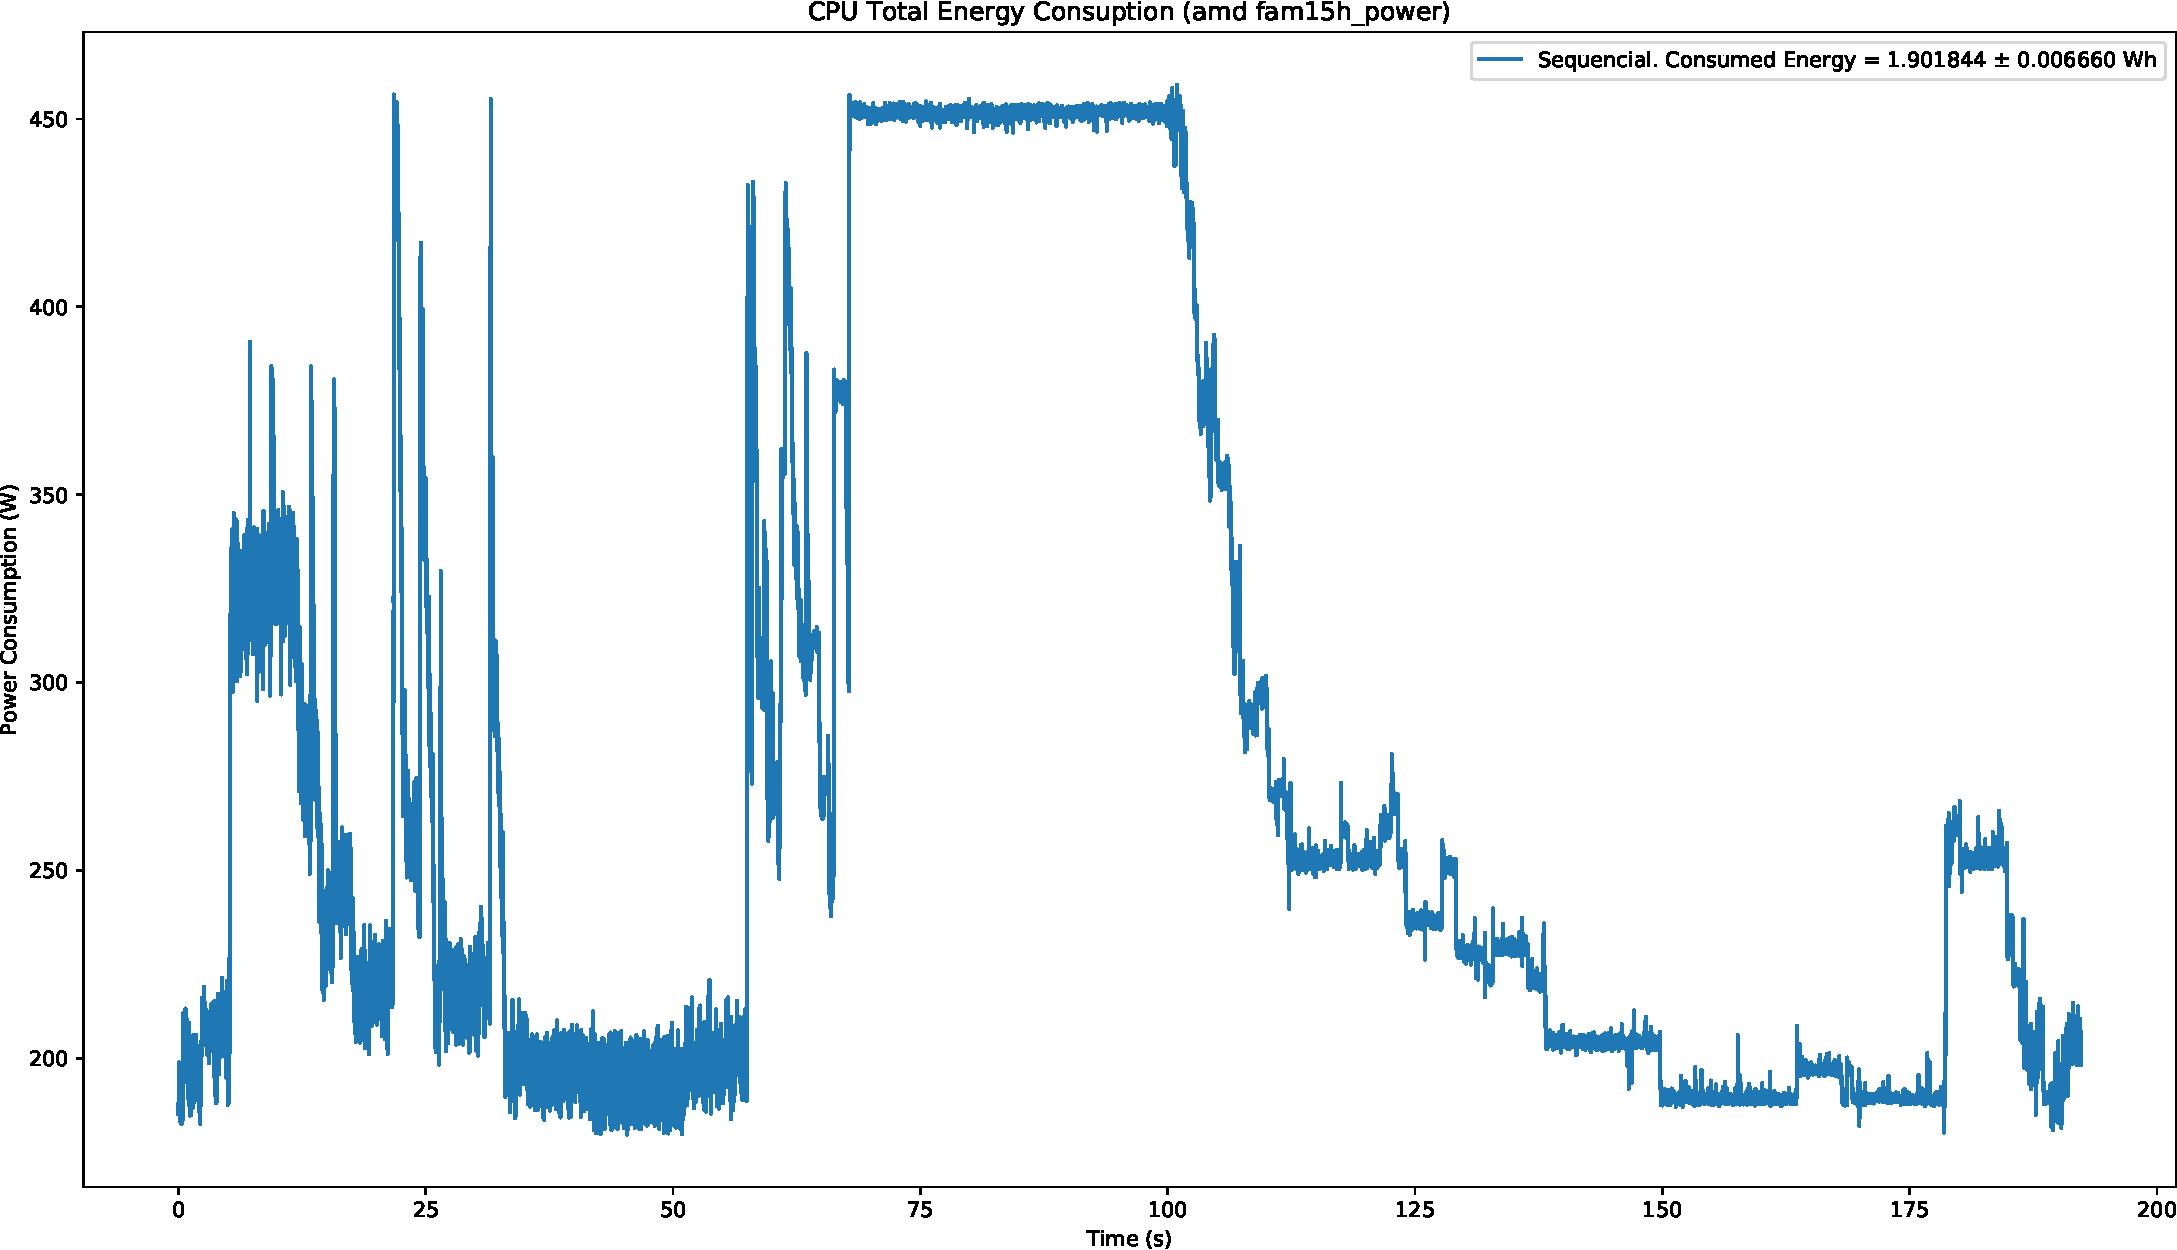
\includegraphics[width=0.9\paperwidth]{sensors-crop.pdf}
    %   \captionof{figure}{Tempo corrido na compilação do GCC em um processador de
    %64 núcleos. \textbf{Sem} LTO, sem \textit{Bootstrap}.}
    \label{fig:analysis_classical}
\end{frame}

\begin{frame}[standout]
    Usando o \texttt{LTO}
\end{frame}

\begin{frame}{Processo de Compilação Usando o LTO}

\begin{figure}
\tikzstyle{block} = [rectangle, draw, fill=white,
    text width=6em, text centered, rounded corners, node distance=1cm and 1cm, auto, minimum height=2em]
\tikzstyle{line} = [draw, -latex, node distance=1cm and 1cm, auto]
\tikzstyle{cloud} = [draw, ellipse,fill=white, node distance=2cm,
    minimum height=2em]
\begin{center}
\scalebox{0.6}{
\begin{tikzpicture}
    % Place nodes
    \node [block]                         (make)   {Makefile};
    \coordinate[below=of make]            (c);
    \node [block, left=of c]              (fonte1) {fonte1.c};
    \node [block, right=of fonte1]        (fonte2) {fonte2.cpp};
    \node [block, right=of fonte2]        (fonte3) {fonte3.f90};

    \node [block, below=of fonte1]        (gcc)      {gcc};
    \node [block, below=of fonte2]        (g++)      {g++};
    \node [block, below=of fonte3]        (gfortran) {gfortran};

    \node [block, below=of gcc]           (objeto1) {lto\_obj1.o};
    \node [block, below=of g++]           (objeto2) {lto\_obj2.o};
    \node [block, below=of gfortran]      (objeto3) {lto\_obj3.o};

    \node [block, below=of objeto2]       (gcc_lto) {gcc\_lto1};

    \node [block, right=of fonte3]       (gcc_wpa) {gcc\_wpa};
    \coordinate[below=of gcc_wpa]            (c2);

    \node [block, left=of c2, right=of gfortran]            (gcc_ltrans1) {gcc\_ltrans};
    \node [block, right=of gcc_ltrans1]   (gcc_ltrans2) {gcc\_ltrans};
    \node [block, right=of gcc_ltrans2]   (gcc_ltrans3) {gcc\_ltrans};

    \node [block, below=of gcc_ltrans1]   (obj1) {obj1.o};
    \node [block, below=of gcc_ltrans2]   (obj2) {obj2.o};
    \node [block, below=of gcc_ltrans3]   (obj3) {obj3.o};

    \node [block, below=of obj2]   (ld) {LD};

	\node [block, below=of ld]  (bin) {Executável};


    \coordinate[right=of objeto3, left=of obj1]    (c3) at (8.2, -5);

    % Draw edges
    \draw[->]    ([xshift=-0.7em] make.south)   -- (fonte1.north);
    \draw[->]    (make.south)   -- (fonte2.north);
    \draw[->]    ([xshift=+0.7em] make.south)   -- (fonte3.north);

    \draw[->]    (fonte1.south)   -- (gcc.north);
    \draw[->]    (fonte2.south)   -- (g++.north);
    \draw[->]    (fonte3.south)   -- (gfortran.north);

    \draw[->]    (gcc.south)   -- (objeto1.north);
    \draw[->]    (g++.south)   -- (objeto2.north);
    \draw[->]    (gfortran.south)   -- (objeto3.north);

    \draw[->]    (objeto1.south)   -- ([xshift=-0.7em]gcc_lto.north);
    \draw[->]    (objeto2.south)   -- (gcc_lto.north);
    \draw[->]    (objeto3.south)   -- ([xshift=+0.7em]gcc_lto.north);

    \draw        (gcc_lto.east)   to [out=0, in=-90] (c3);
    \draw[->]    (c3.north)       to [out=90, in=180] (gcc_wpa.west);

    \draw[->]    (gcc_wpa.south)   -- (gcc_ltrans1.north);
    \draw[->]    (gcc_wpa.south)   -- (gcc_ltrans2.north);
    \draw[->]    (gcc_wpa.south)   -- (gcc_ltrans3.north);

    \draw[->]    (gcc_ltrans1.south)   -- (obj1.north);
    \draw[->]    (gcc_ltrans2.south)   -- (obj2.north);
    \draw[->]    (gcc_ltrans3.south)   -- (obj3.north);

    \draw[->]    (obj1.south)   -- ([xshift=-0.7em]ld.north);
    \draw[->]    (obj2.south)   -- (ld.north);
    \draw[->]    (obj3.south)   -- ([xshift=+0.7em]ld.north);

	\draw[->]    (ld.south)   -- (bin.north);


\end{tikzpicture}
}
\end{center}
\caption{Compilação de um programa utilizando LTO.}
\label{fig:whopr_build}
\end{figure}
\end{frame}


\begin{frame}
    Paralelismo com LTO
    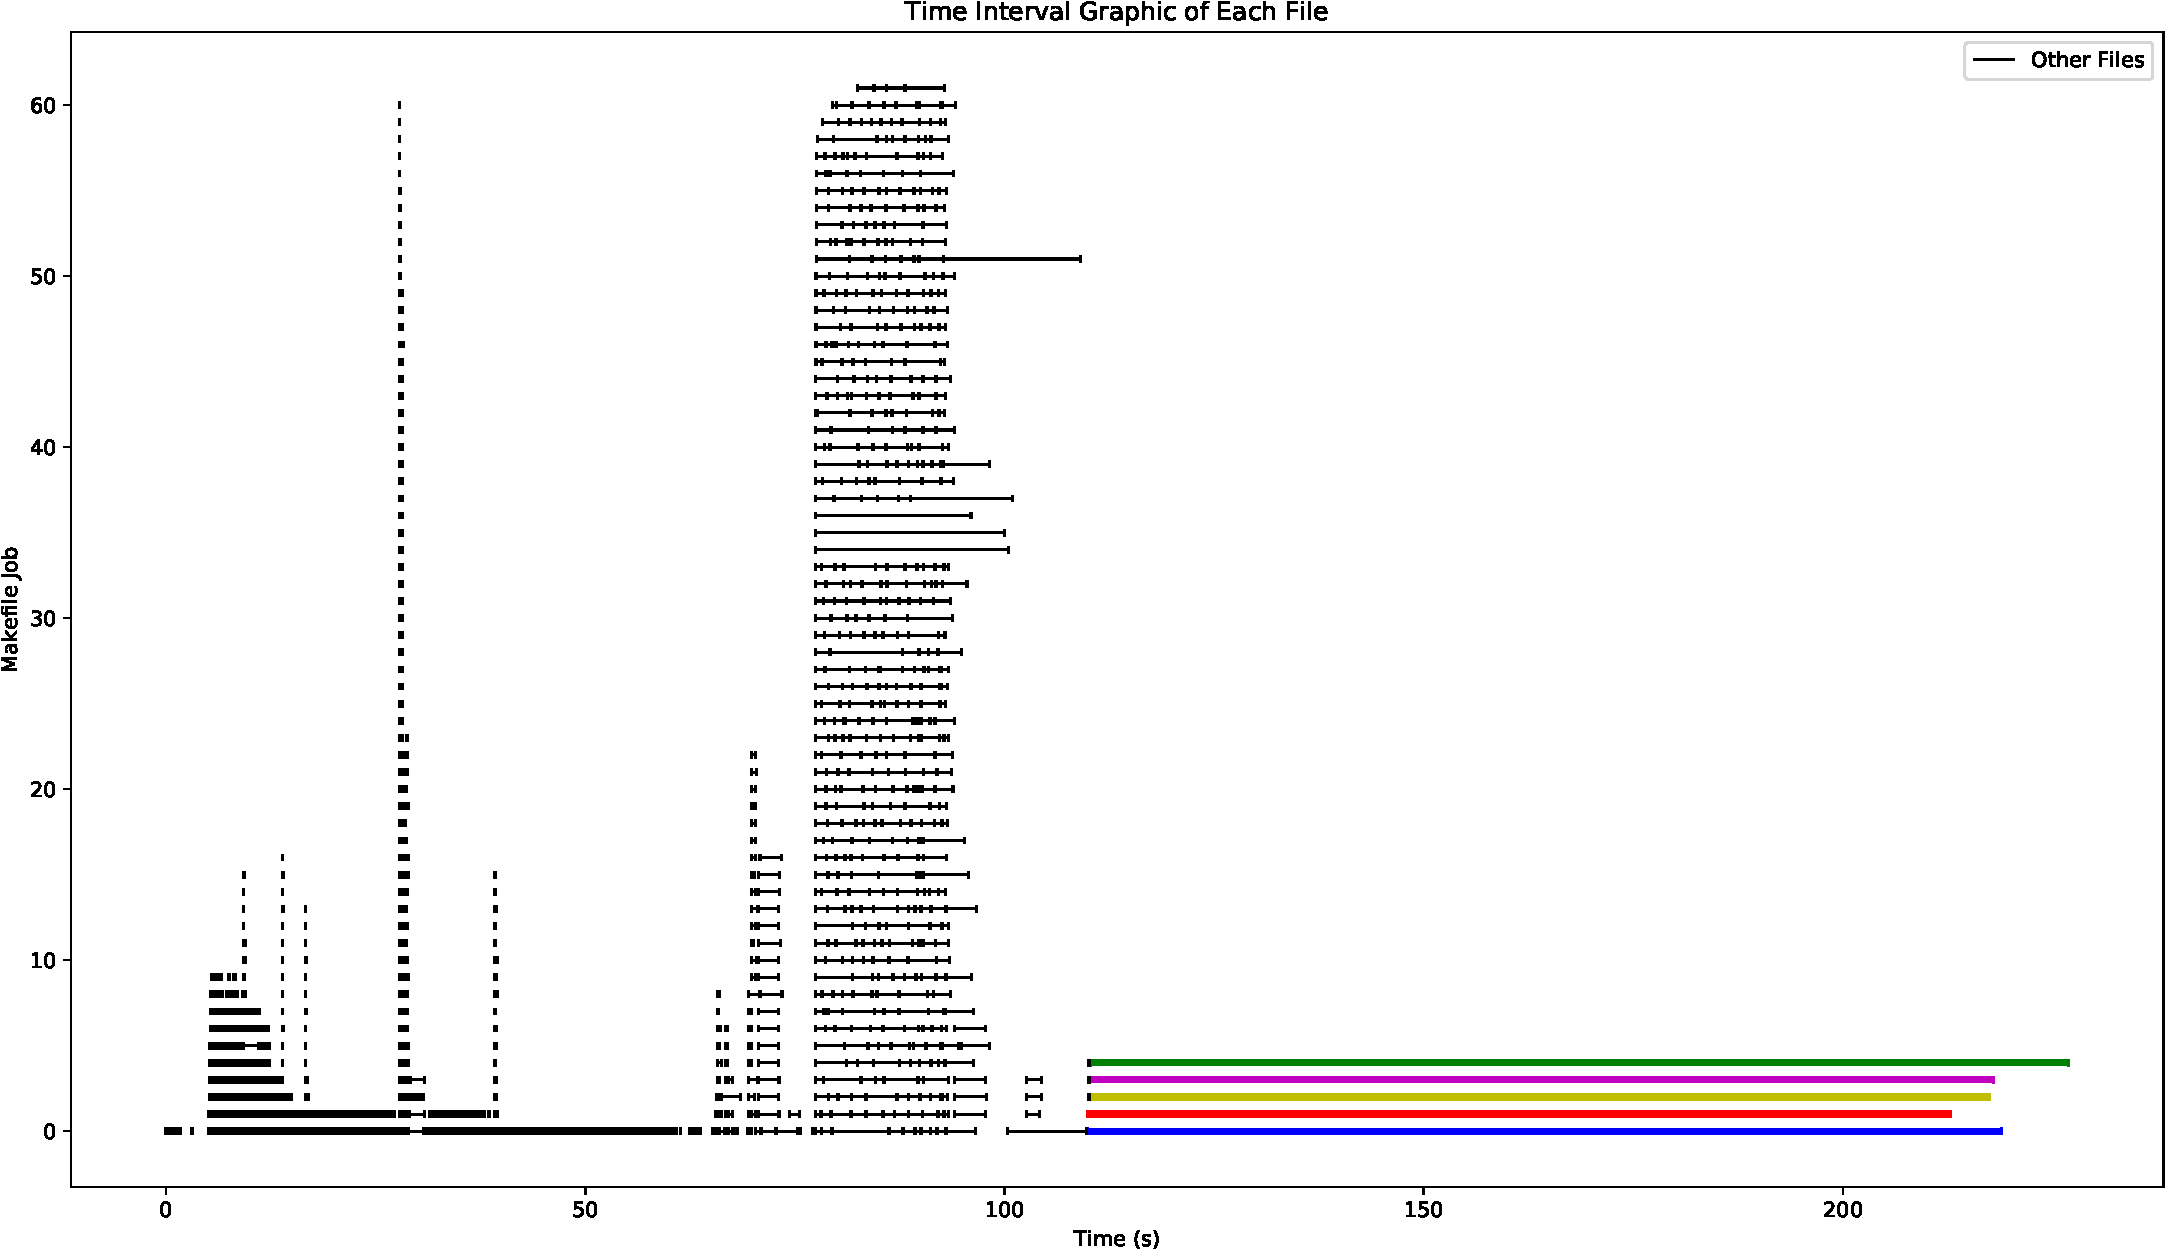
\includegraphics[width=0.9\paperwidth]{lto_crop.pdf}
    %   \captionof{figure}{Tempo corrido na compilação do GCC em um processador de
    %64 núcleos. \textbf{Sem} LTO, sem \textit{Bootstrap}.}
    \label{fig:analysis_lto}
\end{frame}

\begin{frame}[fragile]{Problematização}
    Problemas na \texttt{libcairo}

\begin{verbatim}

Schlachter 2014-08-01 21:31:36 UTC

commit c7ff9bb32e20679d6da4e8a2856be716e5bd9e12
Author: Uli Schlachter <psychon@znc.in>
Date:   Mon Jul 21 17:10:16 2014 +0200

    Remove LTO support

    This just never worked too well and caused too many issues.
    I don't think anyone will miss this.

\end{verbatim}

\end{frame}

\begin{frame}{Problematização}
    Desempenho dos Binários em LTO \citep{Johnson:2017:TSI:3049832.3049845}
    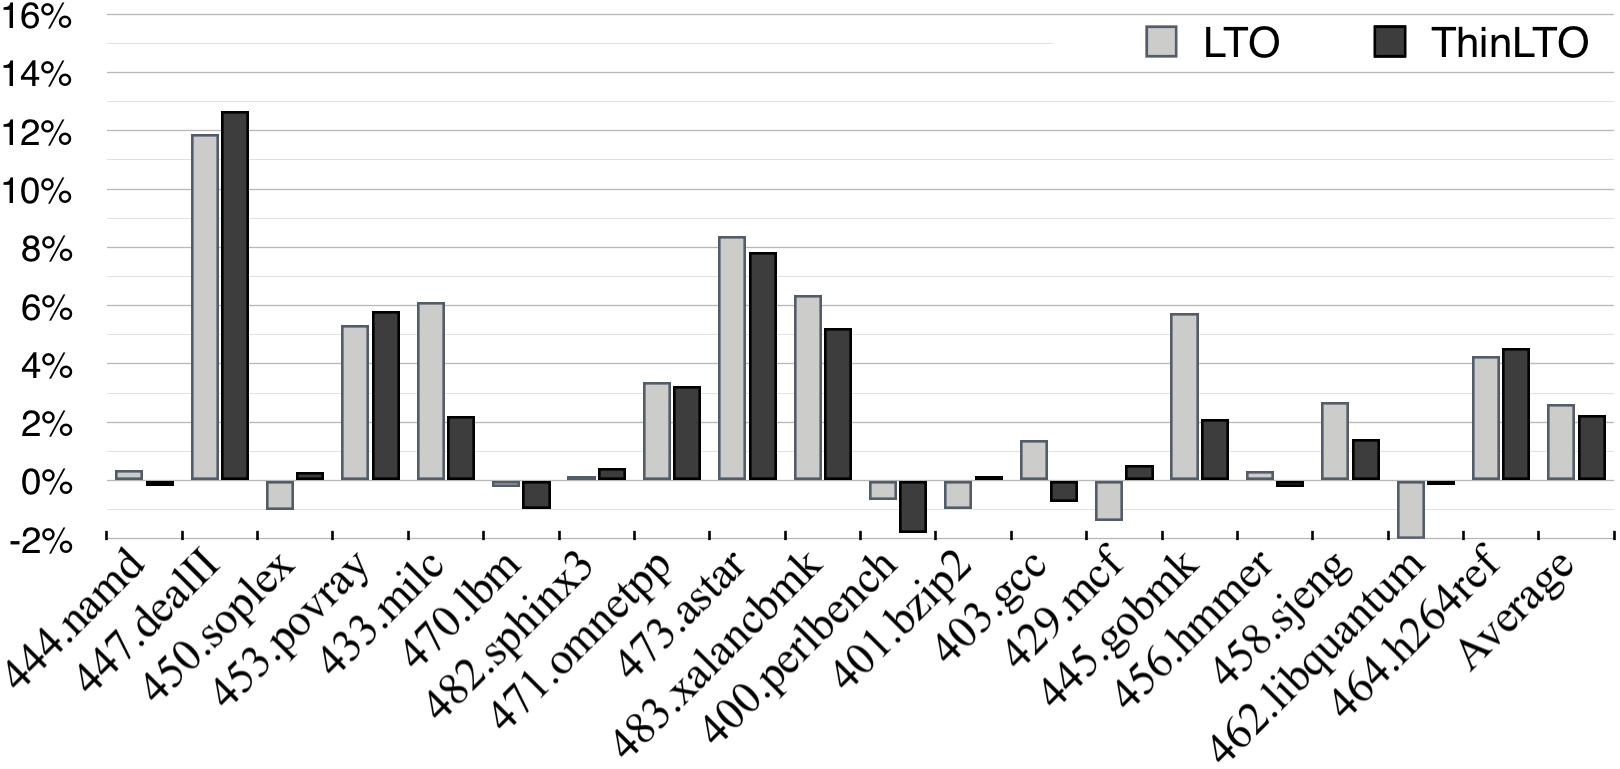
\includegraphics[width=0.9\paperwidth]{LTO_vs_ThinLTO_vs_default.png}
    %   \captionof{figure}{Tempo corrido na compilação do GCC em um processador de
    %64 núcleos. \textbf{Sem} LTO, sem \textit{Bootstrap}.}
    \label{fig:performance_lto}
\end{frame}

\begin{frame}[standout]
    Crescimento do Poder Computacional
\end{frame}

\begin{frame}{Problematização}
    Crescimento do Poder Computacional \citep{42years}

    \centering
    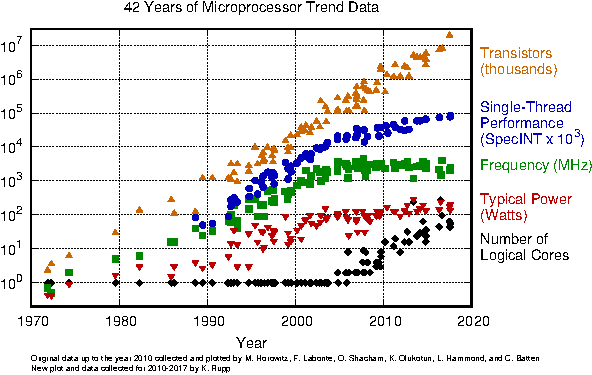
\includegraphics[scale=1.0]{42-years-processor-trend.pdf}
    \label{fig:42years}
\end{frame}

\section{Estado Atual da Pesquisa}

\begin{frame}{Estado Atual da Pesquisa}
    \begin{itemize}
        \item Estudo do gargalo na compilação do GCC usando o \texttt{gimple-match.c}
            \begin{itemize}
                \item São necessários em média 76 segundos para compilar tal arquivo
                \item 75\% ($57s$) é gasto em otimizações Intra Procedurais e Geração de código
                \item 11\% ($11s$) é gasto nas otimizações Inter Procedurais
                \item 8\% ($6s$) é gasto na análise léxica e sintática
                \item 1\% está distribuído em diversas partes do compilador
            \end{itemize}
    \end{itemize}
\end{frame}

\begin{frame}{Estado Atual da Pesquisa}
    \begin{itemize}
        \item Estudo do gargalo na compilação do GCC usando o \texttt{gimple-match.c}
            \begin{itemize}
                \item Se paralelizarmos a aplicação das otimizações Intra Procedurais
            \begin{itemize}
                \item $T_1$: tempo sequencial \hfil\hfil $T_p$: Tempo paralelo com $p$ processadores
                \item Usando a Lei de Amdahl:
$$ T_p = \frac{1}{4} T_1 + \frac{3}{4p}T_1 = \frac{1}{4} \left( 1 + \frac{3}{p}
\right)T_1 $$ 
                \item O \textit{speedup} máximo por arquivo é: $$
\lim_{p \rightarrow +\infty} \frac{T_1}{T_p} = \lim_{p \rightarrow +\infty}
\frac{T_1}{\frac{1}{4} \left( 1 + \frac{3}{p} \right)T_1} = \lim_{p \rightarrow
+\infty} \frac{4}{1 + \frac{3}{p}} = 4$$
            \end{itemize}
            \end{itemize}
    \end{itemize}
\end{frame}


\begin{frame}{Estado Atual da Pesquisa}
    \begin{itemize}
        \item Estratégia corrente para paralelizar a aplicação das otimizações Intra-Procedurais
            \begin{itemize}
                \item Maneira similar ao trabalho de \cite{wortman1992}
                \item Execução de um número fixo de \textit{threads}
                \item O IPA alimenta as funções do programa em uma fila no fim de sua análise
                \item Cada \textit{thread} é responsável por retirar o seu trabalho da fila
                \item Implementação atual consome $0.1s$ para gerenciar $2000$ funções.
    \end{itemize}
\end{itemize}

 \centering
 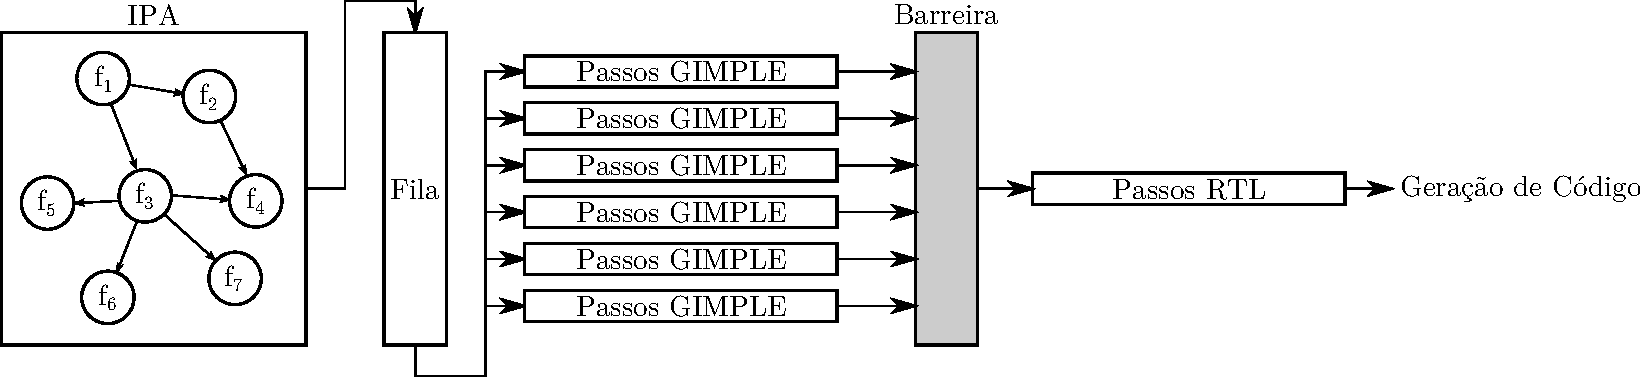
\includegraphics[width=\textwidth]{paralelizacao.pdf}
\end{frame}

\begin{frame}{Estado Atual da Pesquisa}
    \begin{itemize}
        \item Mapeamento de variáveis globais e dependências falsas no GCC
            \begin{itemize}
                \item Variáveis compartilhadas no IPA e nas Otimizações Intra Procedurais
                \begin{itemize}
                    \item Algumas transferidas para a instância objeto que representa as funções do programa
                \end{itemize}
                \item Separação dos passos IPA, GIMPLE e RTL
                \item Fazer ``\textit{troca de contexto}'' das funções não faz mais o compilador abortar com erro!
                \item Enfrentando problemas com o alocador de memória
                \begin{itemize}
                    \item Solução paliativa é travar um \textit{mutex} toda vez que for alocar memória
                \end{itemize}
    \end{itemize}
\end{itemize}
\end{frame}

\section{Metodologia de Validação}

\begin{frame}{Metodologia de Validação}
    \begin{itemize}
        \item Técnicas de inferência estatística medição de tempo
            \begin{itemize}
                \item Distribuição Probabilística do tempo de compilação
                \item Teorema do Limite Central
                \item Intervalos de Confiança
            \end{itemize}
        \item Técnica para verificação de corretude
            \begin{itemize}
                \item Execução dos 62180 testes do GCC
                \item \textit{Bootstrap} (compilar a si mesmo)
            \end{itemize}
        \item Técnica para cálculo de Energia Consumida
        \begin{itemize}
            \item Uso do sensor \texttt{amd fam15h\_power}
            \begin{itemize}
                \item Mede a potência instantânea enviada à CPU pela \textit{Northbridge}
            \end{itemize}

            \item Definição de Potência Instantânea
            \item Integral numérica
            \item Teorema do Confronto
        \end{itemize}
    \end{itemize}
\end{frame}

\section{Referências}

\begin{frame}[allowframebreaks]{Referências}
  %\nocite{bronevetsky02, schmidt03:MSc, FSF:GNU-GPL, CORBA:spec, MenaChalco08, natbib, biblatex, eco:09}
  \printbibliography
\end{frame}

% Recapitulando
\begin{frame}{Tópicos em Paralelização de Compiladores}
  \overview

  % \begin{center} acrescenta espaço vertical;
  % como possivelmente temos bem pouco espaço aqui,
  % vamos usar centering
  {%
    \centering\noindent%
    \url{https://github.com/giulianobelinassi/gcc-timer-analysis}\par
    \url{https://gitlab.com/flusp/gcc/tree/giulianob\_parallel}\par
  }

\end{frame}

\begin{frame}[standout]
    Obrigado!
\end{frame}

\appendix

\begin{frame}{Teorema do Limite Central}
    \begin{itemize}
        \item Seja $(X_1, X_2, \dots, X_n)$ amostras de uma variável aleatória $X$ com média
            $\mu$ e desvio padrão $\sigma$. Então
            $$ Z = \frac{\overline{X} - \mu}{\sigma / \sqrt{n}} \sim N(0, 1)$$
        \item Ou seja, a distribuição do erro $e = \overline{X} - \mu$ segue uma distribuição $N(0, \sigma^2/n)$
        \item Problema: não sei ao certo o valor de $\sigma$ da população
    \end{itemize}
\end{frame}

\begin{frame}{Teorema do Limite Central}
    \begin{itemize}
        \item No caso em que $X \sim N(\mu, \sigma^2)$, então é possível usar o estimador
            $$s^2 = \frac{1}{n-1}\sum_{i=1}^n (X_i - \overline{X})^2$$
        \item Nesse caso
            $$ T = \frac{\overline{X} - \mu}{s / \sqrt{n}} \sim t_{n-1}$$
    \end{itemize}
\end{frame}

\begin{frame}{Cálculo de Energia Consumida}
    \begin{itemize}
        \item Definição de Potência Instantânea:
            $$P(t) = \frac{dE}{dt}$$
        \item Solução da Eq. Diferencial para $E(t)$
            $$E = \int_{t_0}^{t_1} P(t) dt$$

        \item Não é possível calcular essa integral com precisão absoluta no computador
            \begin{itemize}
                \item Temos apenas amostras de $P(t)$
                \item Estratégia: encontrar um limitante inferior e outro superior para $E$
            \end{itemize}
    \end{itemize}
\end{frame}

\begin{frame}{Cálculo de Energia Consumida}
    \begin{itemize}
        \item Discretizando $dt$ em $\Delta t = t_{i+1} - t_{i}$ com $n$ pontos, define:
            $$p_i = \inf\{P(t)\,|\,t_{i} \leq t \leq t_{i+1}\}$$
            \hfil\hfil e \hfil\hfil
            $$P_i = \sup\{P(t)\,|\,t_{i} \leq t \leq t_{i+1}\}$$
            \hfil\hfil então: \hfil\hfil
            $$\sum_{i=1}^{n-1} p_i\Delta t \leq E \leq \sum_{i=1}^{n-1} P_i\Delta t$$

    \end{itemize}
\end{frame}
